In the general case, the calculation of the interaction of a high-intensity laser pulse with a group of dense spherical clusters located in three-dimensional space requires long and complex non-stationary calculations due the changes of the electron density of clusters in time. To check the scale of such change, we simulated the evolution of the electron density distribution for single one-dimensional cluster using LPIC++~\cite{Pfund1998}.

\begin{tikzfigure}
    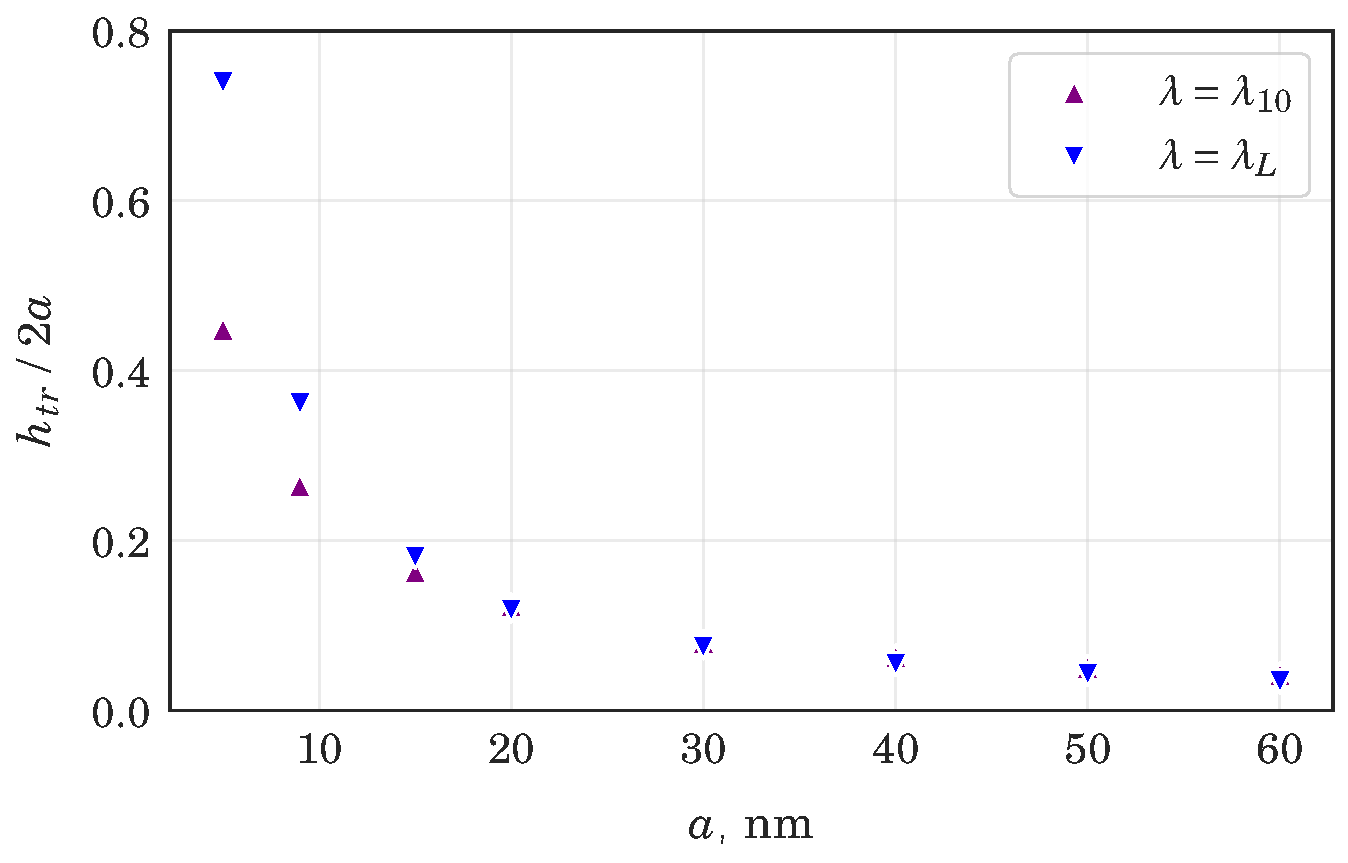
\includegraphics[width=0.6\linewidth]{../img/lpic/htr_over_2a_a}\label{lpic_htr:image}\caption{Asymptotic behavior of the average total thickness of the transition layer at $0 \leq t \leq 10T$ with respect to the target radius. $n_c$ used in the construction corresponds to the critical density for the wavelength $\lambda = \lambda_{10}$.}
\end{tikzfigure}